\documentclass{beamer}
\usetheme{Madrid}

\usepackage{amsmath, amssymb, amsthm}
\usepackage{graphicx}
\usepackage{listings}
\usepackage{gensymb}
\usepackage[utf8]{inputenc}
\usepackage{hyperref}
\usepackage{gvv}
\usepackage{tikz}
\usepackage{minted}
\usetikzlibrary{decorations.pathmorphing}

\begin{document}
\title{MATGEO - 1.10.28}
\author{AI24BTECH11034 - Tanush Sri Sai Petla}
\date{}
\frame{\titlepage}

\begin{frame}{Question}
Write down a unit vector in XY-plane, making an angle of $30\degree$ with the positive direction of X-axis.
\end{frame}

\begin{frame}{allowframebreaks}
\frametitle{Terms Used}
\begin{table}[htbp]
    \centering
    \caption{Terms used}
    \label{tab:parameters}
    \begin{tabular}[12ptx]{ |c| c|}
    \hline\textbf{Term} & \textbf{Description}\\
    \hline
    $\alpha$&Angle made by the vector with positive X-axis \\
    \hline
    $\beta$&Angle made by the vector with positive Y-axis \\
    \hline
    $m$&unit direction vector\\
    \hline
    \end{tabular}
\end{table}
\end{frame}
\begin{frame}{Solution}
In the 2D space, the unit direction vector is defined as\\
\begin{equation}
    m=\begin{pmatrix}
        \cos\alpha\\
        \cos\beta\\
    \end{pmatrix}
\end{equation}
Where $\alpha.\beta$ are the angles made by the vectors with the axes.

Angle made by the unit vector in question with the positive X-axis and positive Y-axis $\colon$\\
\begin{equation}
    \alpha=30\degree
\end{equation}
\begin{equation}
    \beta=60\degree
\end{equation}
\end{frame}
\begin{frame}{Solution}
From equation 1, the required unit vector is$\colon$
\begin{equation*}
    \begin{pmatrix}
        \frac{\sqrt{3}}{2}\\
        \frac{1}{2}
    \end{pmatrix}
\end{equation*} 
\end{frame}

\begin{frame}{Plot}
    \begin{center}
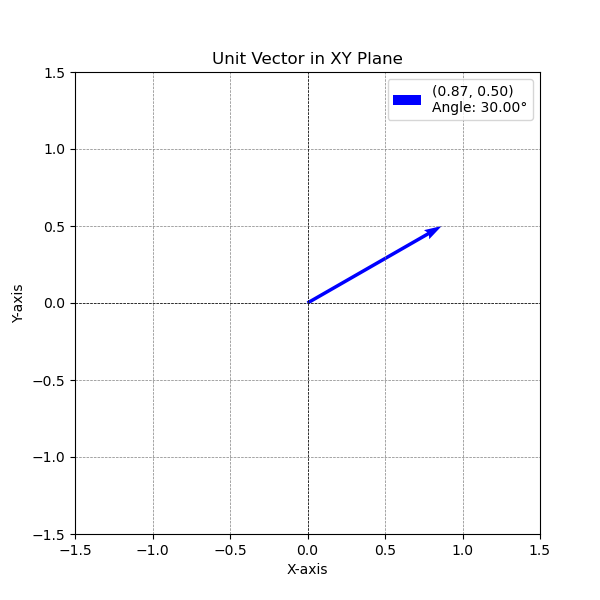
\includegraphics[width=0.6\textwidth]{figs/figure1.png}
\end{center}
\end{frame}

\begin{frame}[fragile]
\frametitle{Python code for graph}
\begin{minted}[linenos=true]{python}
import numpy as np
import matplotlib.pyplot as plt

# Read the unit vector from the output.txt file
with open('output.txt', 'r') as file:
    line = file.readline()
    x, y = map(float, line.split())

# Calculate the angle of the vector in degrees
angle = np.degrees(np.arctan2(y, x))

# Plotting the vector
plt.figure(figsize=(6, 6))
plt.quiver(0, 0, x, y, angles='xy', scale_units='xy', scale=1, 
color='b', label=f'({x:.2f}, {y:.2f})\nAngle: {angle:.2f}°')
\end{minted}
\end{frame}
\begin{frame}[fragile]
\frametitle{Python code for graph}
\begin{minted}[linenos=true]{python}
plt.xlim(-1.5, 1.5)
plt.ylim(-1.5, 1.5)
plt.axhline(0, color='black', linewidth=0.5, ls='--')
plt.axvline(0, color='black', linewidth=0.5, ls='--')
plt.grid(color='gray', linestyle='--', linewidth=0.5)

plt.title('Unit Vector in XY Plane')
plt.xlabel('X-axis')
plt.ylabel('Y-axis')

# Adding a legend
plt.legend(loc='upper right')

# Save the plot as figure1.png
plt.savefig('figure1.png')
plt.show()
\end{minted}
\end{frame}
\end{document}
